\documentclass[10pt,a4paper]{article}
\usepackage{rpgcover}
\usepackage{illustrated-panel}
\usepackage{longtable,booktabs}
\usepackage{float}
\usepackage{multicol}
\usepackage{fancyvrb}
\usepackage{wrapfig}
\usepackage{needspace}
\usepackage{titlesec}
\babelprovide[import]{french}
\titleformat{\subsection}{\normalfont\Large\bfseries\color{rpgbrown}}{}{0pt}{}
\titlespacing*{\subsection}{0pt}{12pt plus 2pt}{5pt}
\titleformat{\subsubsection}{\normalfont\normalsize\bfseries\color{rpgbrown}}{}{0pt}{}
\titlespacing*{\subsubsection}{0pt}{10pt plus 2pt}{4pt}
\usepackage{etoolbox}
% Stat boxes never start in the last lines of a page, where they would split after their title.
\BeforeBeginEnvironment{rpgnote}{\par\needspace{8\baselineskip}}
\pretocmd{\subsection}{\needspace{5\baselineskip}}{}{}
\pretocmd{\subsubsection}{\needspace{4\baselineskip}}{}{}
\setcounter{tocdepth}{1}
\clubpenalty=10000
\widowpenalty=10000
\displaywidowpenalty=10000
\interlinepenalty=0
\emergencystretch=1.2em
\newcommand{\HHInlineFigure}[3]{%
  \begin{center}\includegraphics[width=#2\linewidth,height=56mm,keepaspectratio]{assets/hollow-hearth/#1.jpg}%
  \par\vspace{2pt}{\footnotesize\itshape\color{rpgbrown}#3\par}\end{center}}
% Scene-opening illustrations float: here when they fit, otherwise at the foot of the next page.
% They never narrow a read-aloud box or leave a gap at the bottom of a page.
\newcommand{\HHSceneArt}[2]{%
  \begin{figure}[!hb]\centering\includegraphics[width=.62\linewidth,height=58mm,keepaspectratio]{assets/hollow-hearth/#1.jpg}%
  \par\vspace{2pt}{\footnotesize\itshape\color{rpgbrown}#2\par}\end{figure}}
% Full-page maps float to the next free page instead of ending the current page early.
\newcommand{\HHSceneMap}[3]{%
  \begin{figure}[p]\centering
    {\Large\bfseries\color{rpgbrown}#2\par}\vspace{6mm}%
    \includegraphics[width=.96\linewidth,height=190mm,keepaspectratio]{assets/hollow-hearth/#1.jpg}\par\vspace{4mm}%
    {\small\itshape\color{rpgbrown}#3\par}%
  \end{figure}}
\newcommand{\HHContents}{%
  \clearpage\thispagestyle{rpg}
  \vspace*{10mm}\begin{center}{\fontsize{27}{31}\selectfont\bfseries SOMMAIRE\par}\vspace{9pt}
  {\color{rpgline}\rule{.76\linewidth}{.55pt}}\end{center}\vspace{9mm}
  \begingroup
  \expandafter\def\csname l@section\endcsname##1##2{\csname @dottedtocline\endcsname{1}{0em}{4em}{\bfseries ##1}{##2}}%
  \csname @starttoc\endcsname{toc}\endgroup
  \vspace{5mm}
  \begin{center}
\includegraphics[height=68mm,width=.59\linewidth,keepaspectratio]{assets/hollow-hearth/front-overlay.png}\end{center}
  \vfill
  \begin{center}{\small\itshape Une aventure de Jacopo Biscella\par}\vspace{5pt}
  {\footnotesize Cette aventure est diffusée sous licence Creative Commons Attribution — Partage dans les mêmes conditions 4.0 International (CC BY-SA 4.0), comme Au dernier lancer. Vous pouvez la partager et l’adapter, y compris commercialement, en créditant l’auteur et en conservant la même licence.\par}\end{center}
  \clearpage}
\RPGSetRunningTitle{La cloche de l’Âtre Creux}
\RPGSetCoverWordSpace{.78em}
\hypersetup{pdftitle={La cloche de l’Âtre Creux},pdfauthor={Jacopo Biscella}}
\setlength{\emergencystretch}{2em}
\setcounter{secnumdepth}{-1}
\newcommand{\tightlist}{\setlength{\itemsep}{0pt}\setlength{\parskip}{0pt}}

\newcommand{\HHFrontArt}{assets/hollow-hearth/front-overlay.png}
\newcommand{\HHBackArt}{assets/hollow-hearth/back-overlay.png}
% Existing rpgcover.sty is used unchanged; only an adventure-specific back-cover layout follows.

\setlength{\parskip}{2pt plus .5pt minus .5pt}
\linespread{1.025}\selectfont
\newcommand{\HHAdventureBackCover}{%
 \clearpage\pagenumbering{gobble}\RPGCoverPagetrue\thispagestyle{empty}\null
 \begin{tikzpicture}[remember picture,overlay,x=1mm,y=1mm]
  \RPGDrawBackground{\RPGBackBackgroundFile}
  \node[align=center,text=coverink,text width=170mm,inner sep=0pt] at ($(current page.south west)+(105mm,260mm)$)
    {{\RPGCoverTitleFont\fontsize{19}{23}\selectfont LA CLOCHE DE L’ÂTRE CREUX}};
  \draw[coverink,line width=.45pt] ($(current page.south west)+(57mm,246mm)$)--($(current page.south west)+(153mm,246mm)$);
  \node[anchor=north,align=left,text=coverink,text width=137mm,inner sep=0pt] at ($(current page.south west)+(105mm,240mm)$)
    {\RPGCoverTextFont\fontsize{10.4}{13.4}\selectfont
    Il y a sept générations, un Mystique errant bénit une cloche de bronze. Le village où finit la route du roi et où commence la forêt prit le nom de l’Âtre Creux. Chaque soir, la cloche repoussait le Peuple Creux, des êtres pâles à peau d’écorce qui murmuraient entre les arbres.};
  \node[anchor=north,align=center,text=coverink,text width=140mm,inner sep=0pt] at ($(current page.south west)+(105mm,197mm)$)
    {\RPGCoverSubtitleFont\fontsize{13}{17}\selectfont Il y a trois nuits, la cloche a été volée.\\[4pt]
    La prochaine nuit sans lune aura lieu dans quarante-huit heures.};
  \draw[coverink,line width=.45pt] ($(current page.south west)+(57mm,167mm)$)--($(current page.south west)+(153mm,167mm)$);
  \node[anchor=north,align=left,text=coverink,text width=137mm,inner sep=0pt] at ($(current page.south west)+(105mm,162mm)$)
    {\RPGCoverTextFont\fontsize{9.9}{12.1}\selectfont
    Une aventure d’initiation pour Au dernier lancer, destinée à trois ou quatre Protagonistes et jouée en deux ou trois heures. Elle présente les niveaux de dés, les distances narratives, les Blessures, la Fatigue, la magie et le Contrecoup.};
  \node[anchor=north,align=center,text=coverink,text width=147mm,inner sep=0pt] at ($(current page.south west)+(105mm,133mm)$)
    {\RPGCoverSubtitleFont\fontsize{10.5}{13.2}\selectfont
     Trois approches. Une fin choisie par le groupe.\\
     Un chevalier déshonoré. Un acheteur mystérieux.\\
     Une décision à prendre ensemble.};
  \node[anchor=north,align=center,text=coverink,text width=144mm,inner sep=0pt] at ($(current page.south west)+(105mm,114mm)$)
    {\RPGCoverTextFont\fontsize{10.2}{12.5}\selectfont
     Contient~: quatre cartes $\cdot$ cinq illustrations $\cdot$\\ un aide-mémoire pour le Narrateur.};
  \RPGOptionalArtwork{105}{59}{130}{24}{\HHBackArt}
  \filldraw[fill=white,draw=coverink,line width=.55pt]
    ($(current page.south west)+(139mm,25mm)$) rectangle
    ($(current page.south west)+(187mm,55mm)$);
 \end{tikzpicture}
 \clearpage\RPGCoverPagefalse
}
\newcommand{\HHFrontCover}{%
 \clearpage\RPGCoverPagetrue\thispagestyle{empty}\null
 \begin{tikzpicture}[remember picture,overlay,x=1mm,y=1mm]
  \RPGDrawBackground{\RPGFrontBackgroundFile}
  \node[align=center,text=coverink,text width=138mm,inner sep=0pt]
   at ($(current page.south west)+(105mm,248mm)$)
   {\RPGCoverTitleFont\fontsize{16.6}{20.7}\selectfont LA CLOCHE DE\\[1.0mm]L’ÂTRE CREUX};
  \node[align=center,text=coverink,text width=135mm,inner sep=0pt]
   at ($(current page.south west)+(105mm,235mm)$)
   {\RPGCoverSubtitleFont\fontsize{9.5}{12}\selectfont Une aventure pour «~Au dernier lancer~»};
  \RPGOptionalArtwork{105}{119}{150}{138}{\HHFrontArt}
  \node[align=center,text=coverink,text width=124mm,inner sep=0pt]
   at ($(current page.south west)+(105mm,25mm)$)
   {\RPGCoverTextFont\fontsize{12}{15}\selectfont Jacopo Biscella};
 \end{tikzpicture}\clearpage\RPGCoverPagefalse}
\begin{document}
% Select the language here: babel resets to its main language (english) at \begin{document}.
\selectlanguage{french}
\RPGStartFrontMatter
\HHFrontCover
\HHContents
\RPGStartMainMatter
\RPGChapter{La cloche de l’Âtre Creux}
\begin{center}\textit{Une aventure d’initiation pour Au dernier lancer}\par\smallskip
\small 2--3 heures \textperiodcentered\ 3--4 Protagonistes \textperiodcentered\ Au moins un Guerrier \textperiodcentered\ Édition du Narrateur
\end{center}
\noindent\textit{Les quatre Protagonistes prétirés sont publiés avec les téléchargements de cette aventure~: un PDF par fiche, sur le modèle de fiche de personnage du livre de règles.}\par\medskip
\subsection{Un mot au Narrateur}\label{un-mot-au-narrateur}

Cette aventure est d’abord un outil d’apprentissage, et seulement ensuite une histoire. Chaque scène met en avant un pilier précis d’\emph{Au dernier lancer}, sans jamais interrompre la fiction pour faire la leçon. Au moment du générique de fin, vos joueurs auront vécu les jets par niveau, les distances narratives, la réserve commune de Blessures et de Fatigue, l’Aide entre Protagonistes et, si vous faites bien votre travail, au moins un Effort déclaré d’une main tremblante, précisément au moment que promet le titre.

Le rythme visé est à peu près le suivant~:

\begin{itemize}
\tightlist
\item
  30 minutes pour la création des personnages et la mise en place \emph{(utilisez les règles de création du manuel, p.~2--6)}
\item
  35 minutes pour \textbf{Scène 1 · Le village} (enquête sociale)
\item
  40 minutes pour \textbf{Scène 2 · Le bois des murmures} (épreuve de compétences et atmosphère)
\item
  60 minutes pour \textbf{Scène 3 · La vieille tour de guet} (combat final et résolution)
\item
  10 minutes pour \textbf{Les trois questions} et les suites
\end{itemize}

Un rappel qui mérite d’être répété~: dans ce jeu, il n’y a ni jet d’initiative, ni ordre de tour fixe, ni grille. Les cartes fournies avec cette aventure sont des repères spatiaux pour l’imagination de tous~; à la table, les distances sont toujours \textbf{Au contact}, \textbf{Proche}, \textbf{À portée} ou \textbf{Loin}.

\par\vspace{3pt}

\subsection{Ce que cette aventure enseigne}\label{ce-que-cette-aventure-enseigne}

\begingroup\setlength{\arrayrulewidth}{.34pt}\arrayrulecolor{rpgline}\renewcommand{\arraystretch}{1.32}\rowcolors{2}{rpgshade}{white}\par\smallskip\noindent\begin{tabularx}{\linewidth}{|Y|Y}\hline
\rpghead{Scène} & \rpghead{Mécaniques présentées} \\ \hline
Le village & Jets de Caractéristique + Compétence~; SD des actions sociales~; jets opposés~; mise en jeu du Trait et du Fardeau \\ \hline
Le bois des murmures & Aide~; Conditions ($-1$ degré)~; catégories de distance narratives \\ \hline
La vieille tour de guet & Combat~; Blessures et Fatigue~; Critique~; Contrecoup~; \textbf{Effort}~; conséquences \\ \hline
\end{tabularx}\arrayrulecolor{black}\endgroup\par\smallskip

Si le groupe compte un Mystique, c’est aussi dans la scène~3 que son premier Contrecoup risque fort de se produire. Laissez-le arriver.

\par\vspace{3pt}

\par\needspace{65mm}\subsection{Le contexte}\label{les-pruxe9mices}

\begin{wrapfigure}{r}{.38\linewidth}\vspace{-5pt}\centering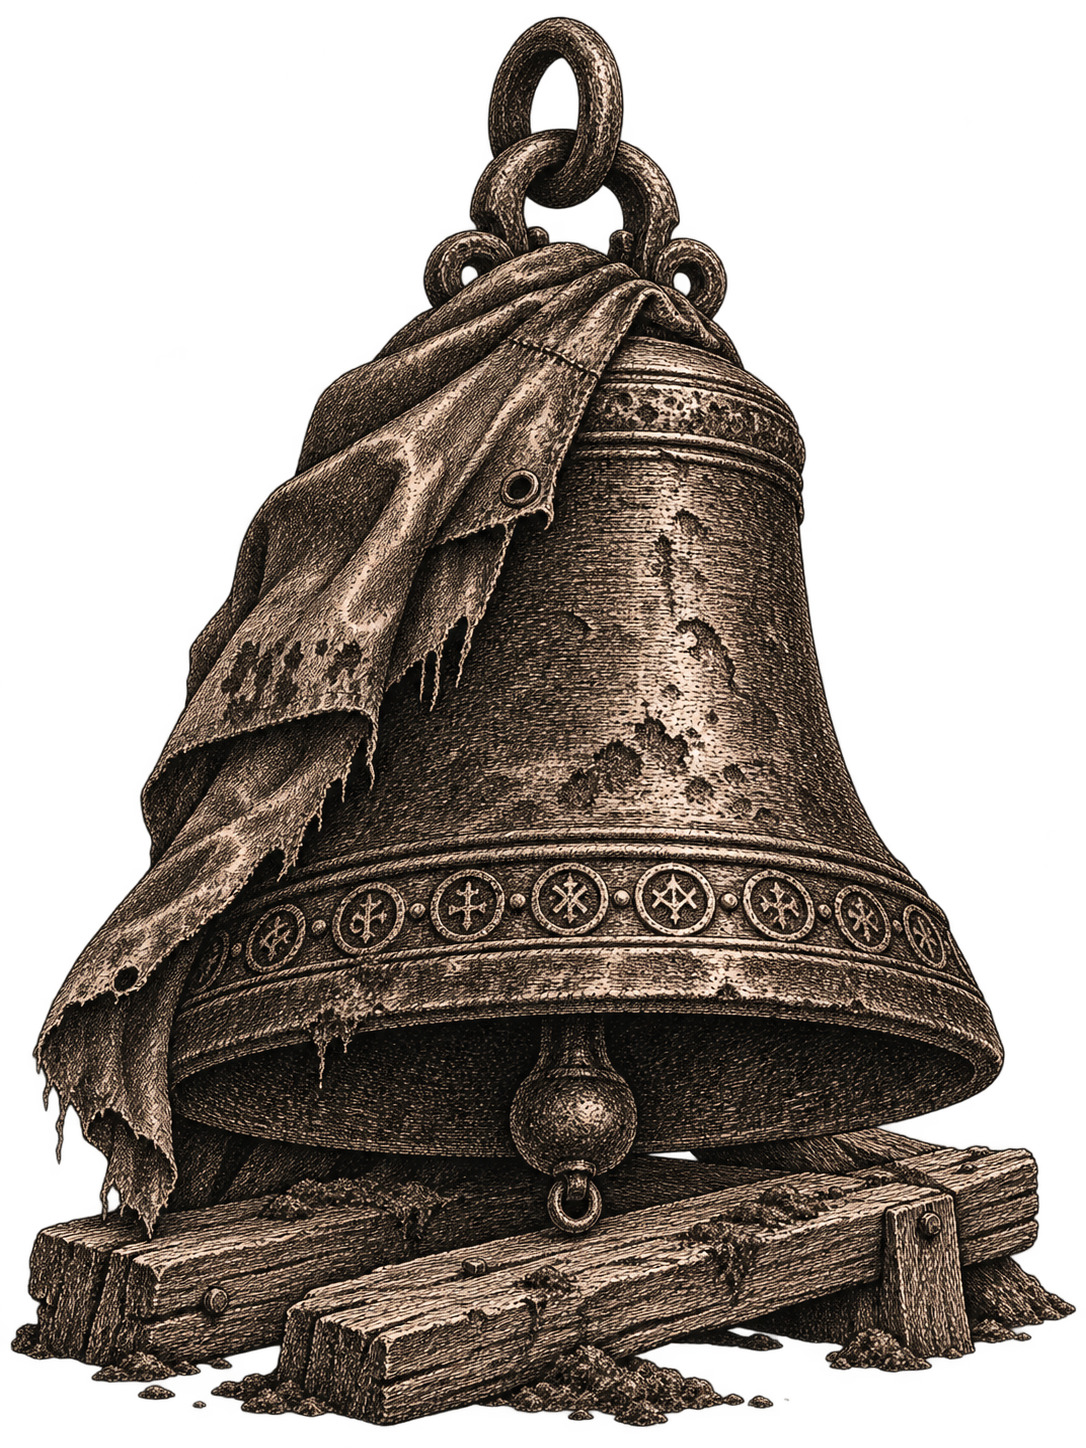
\includegraphics[width=.98\linewidth,height=58mm,keepaspectratio]{assets/hollow-hearth/bell.jpg}\par{\scriptsize\itshape\color{rpgbrown}La cloche volée, enveloppée de toile huilée}\vspace{-5pt}\end{wrapfigure}

Il y a sept générations, un Mystique errant nommé \textbf{Veyl Ashen} bénit une cloche de bronze coulée dans la forge d’un petit village bâti là où s’arrête la route du roi et où commence la vieille forêt. Le village prit le nom de \textbf{l’Âtre Creux}. Sonnée à chaque crépuscule, la cloche maintenait le \textbf{Peuple Creux} --- des êtres pâles à la peau d’écorce, qui murmurent entre les arbres --- parmi les racines, là où est sa place.

Il y a trois nuits, la cloche a été volée.

Une bande de brigands menée par un déserteur nommé \emph{«~Sir~»} \textbf{Corwin Vask} est descendue des ruines de la tour de guet où elle campe, a tué l’apprenti du vieux sonneur, puis a disparu vers le nord dans les bois, la cloche enveloppée de toile huilée. Les villageois ont enterré le garçon hier matin.

La prochaine nuit sans lune tombe dans \textbf{quarante-huit heures}.

Voilà le compte à rebours. Cette nuit-là, une fois la lune couchée, sans cloche pour sonner au crépuscule, le Peuple Creux reviendra dans l’Âtre Creux, un village qui a oublié comment se défendre.

\par\vspace{3pt}

\subsection{L’accroche}\label{laccroche}

\HHSceneArt{village}{L’Âtre Creux au crépuscule~: la plateforme vide}

Adaptez l’arrivée aux Traits et aux Fardeaux que vos joueurs ont écrits. Quelques pistes rapides~:

\begin{itemize}
\tightlist
\item
  Un \textbf{Érudit} qui retrace la lignée de Veyl Ashen dans d’anciens registres liturgiques.
\item
  Un \textbf{Aventurier} porteur d’un contrat de la ville suivante, plus haut sur la route.
\item
  Un \textbf{Mystique} qui a \emph{senti} la cloche se taire, à des lieues de là.
\item
  Un \textbf{Guerrier} qui quitte un champ de bataille où il ne veut plus être.
\end{itemize}

Quelle que soit la route suivie, la maire du village, \textbf{Hesta Thrush}, leur offrira le peu que possède l’Âtre Creux --- quelques pièces, l’hospitalité et une relique conservée depuis la fondation (voir \emph{Résolution}) --- pour qu’ils ramènent la cloche.

\begin{quote}
\subsubsection{À lire à voix haute --- L’arrivée}\label{uxe0-lire-larrivuxe9e}

\emph{La route se réduit à une piste, la piste à un sentier, et le sentier débouche sur une clairière de maisons basses en pierre aux toits d’ardoise pentus. Au centre de la place du village se dresse une plateforme de bois. Vide. Quatre boulons de fer, là où l’on a arraché quelque chose de lourd. Aucune fumée ne monte des cheminées. Il n’y a personne sur la place.}

\emph{Puis une porte s’ouvre, une vieille femme sort et, derrière elle, vous entendez quelqu’un pleurer.}
\end{quote}

\par\vspace{3pt}

\HHSceneMap{map-village}{L’Âtre Creux~: plan du village}{La plateforme de la cloche se dresse sur la place~; Hesta, Bram, Vela et l’auberge sont tout près. Tous les lieux du village~: Proche.}
\RPGChapter{Scène 1 --- Le village}\label{scuxe8ne-1-le-village}

\textbf{Mécaniques en jeu~:} jets de Savoir, bonus de Compétence, jets opposés, mise en jeu du Trait et du Fardeau.

À l’Âtre Creux, trois personnes comptent pour votre enquête. Les Protagonistes peuvent parler aux trois, dans l’ordre qu’ils veulent. Chacune détient une pièce du tableau, et au moins l’une d’elles ment \emph{presque}.

\par\smallskip\begin{rpgnote}[fontupper=\normalfont]\textbf{Personnages du village}\par\smallskip
\textbf{Hesta Thrush} \emph{(PNJ)} --- Savoir Compétent. Pas de statistiques de combat~; si la violence l’atteint, elle n’est que ce qu’elle paraît être.\par\smallskip
\textbf{Vela Roan} \emph{(PNJ)} --- Savoir Expert (Herboristerie, Survie), Merveille Compétent. Ne se bat que si elle est acculée.\par\smallskip
\textbf{Le vieux Bram} \emph{(PNJ)} --- Savoir Compétent. Ne peut plus se battre.\end{rpgnote}\par\smallskip
Consultez \textbf{le plan du village de l’Âtre Creux} pour la disposition des lieux. Tous les lieux du village sont à distance \textbf{Proche} les uns des autres.

\subsubsection{Hesta Thrush --- La maire}\label{hesta-thrush-la-maire}

Une femme d’une soixantaine d’années, le visage tanné par les intempéries, amaigrie par le chagrin. Son fils est parti à la guerre et n’est jamais revenu~; elle est maire depuis onze ans et connaît chaque villageois jusqu’à son deuxième prénom.

Ce qu’elle dit volontiers~:

\begin{itemize}
\tightlist
\item
  Les brigands venaient de la \textbf{vieille tour de guet}, à quatre heures de marche au nord, dans le bois des murmures.
\item
  Elle offre, comme récompense finale du village, une relique de la fondation~: la \textbf{Lame de sel} \emph{(manuel, p.~9)}.
\end{itemize}

Ce sur quoi elle ment~:

Elle sait que son cousin \textbf{Marrel} a été vu en train de boire avec l’un des brigands à l’auberge, la semaine précédant le vol. Elle ne veut pas que son cousin soit pendu pour cela. Un \textbf{jet de Savoir opposé au Savoir (Compétent) d’Hesta} perçoit son malaise. La \textbf{Diplomatie} la convainc de dire la vérité~; la \textbf{Rhétorique} aussi. L’\textbf{Intimidation, SD~5}, fonctionne également, mais retourne le village contre le groupe pour le reste de l’aventure.

\begin{quote}
\subsubsection{Accroche de Trait ou de Fardeau}\label{accroche-de-trait-ou-de-fardeau}

Un Protagoniste dont le Fardeau touche à la guerre, à la perte d’un enfant ou à un serment brisé trouvera en Hesta une alliée ou un miroir. Appuyez-vous dessus. \emph{«~Vous me faites penser à lui~»}, dit-elle en regardant la mauvaise personne.
\end{quote}

\subsubsection{Le vieux Bram --- Le sonneur}\label{le-vieux-bram-le-sonneur}

Le sonneur, plus de quatre-vingts ans, a survécu parce qu’il se soulageait dans les ronces quand les brigands sont arrivés. Le garçon tué était son apprenti et son petit-neveu. Il est en colère. Pas bruyamment. L’autre colère.

Ce qu’il a vu~:

\begin{itemize}
\tightlist
\item
  Quatre hommes. Un en armure, un avec un arc long, deux avec des dagues.
\item
  Celui en armure portait \textbf{un soleil blanc brodé sur l’épaule de son manteau}, l’emblème d’un ordre de chevalerie déshonoré il y a dix ans. Un \textbf{jet de Savoir, SD~4, avec la Compétence Histoire} identifie l’\textbf{Ordre du Soleil Pâle}, dissous pendant les guerres pour «~offenses rituelles~». Sans Histoire, il faut un \textbf{SD~5} pour en exhumer un vague souvenir.
\item
  Il croit que la cloche est vivante. Il a peut-être raison.
\end{itemize}

\subsubsection{Vela Roan --- L’herboriste}\label{vela-roan-lherboriste}

Quarante ans, l’esprit vif, la seule personne du village à être allée \emph{dans} le bois des murmures et à en être revenue. Elle sait ce qu’est le Peuple Creux. Elle ne le dira pas franchement. Elle parle par histoires.

Ce qu’elle offre, si on le lui demande comme il faut~:

\begin{itemize}
\tightlist
\item
  Les «~gens d’écorce~» sortent des racines quand aucune cloche ne sonne. Elle croit qu’un membre du Peuple Creux marche déjà parmi les villageois sous une apparence humaine.
\item
  Elle donnera une fiole de \textbf{racine-de-nuit distillée} --- \emph{un objet remarquable~: versée sur une lame, le coup suivant inflige +1~Blessure contre les créatures surnaturelles~; usage unique} --- \textbf{si} un Protagoniste accepte de lui rapporter un brin de \textbf{fleur d’argent-de-lune} cueilli au cœur des bois.
\end{itemize}

Ce dernier point est une tentation secondaire~: l’occasion d’un moment de Fardeau si quelqu’un manque à sa parole plus tard, ou l’occasion de mettre à l’épreuve un Trait honorable. La fleur existe. Au groupe de décider s’il trouve le temps de la chercher.

\subsubsection{Facultatif · Marrel, le cousin}\label{facultatif-marrel-le-cousin}

Si les Protagonistes creusent le mensonge d’Hesta, ils trouvent Marrel à l’auberge, en train de noyer sa peur dans la boisson. Il confirme que le brigand avec qui il a parlé --- un certain \textbf{Thessik} --- se vantait d’un acheteur qui \emph{«~paie en argent du Nord~»} et qui viendrait chercher la cloche. Marrel ignorait qu’elle serait volée. L’\textbf{Intimidation, SD~4}, le fait craquer. La \textbf{Diplomatie, SD~4}, autour d’un verre, fonctionne aussi. \textbf{Commerce, SD~4}, si un Érudit veut éclaircir ce que signifie vraiment «~argent du Nord~» (c’est un terme employé par les contrebandiers qui passent la frontière~: l’argent du Nord n’existe pas, c’est un code pour l’or des fées).

\subsubsection{Conseil au Narrateur}\label{conseil-au-narrateur}

Quand un joueur déclare \emph{«~Je veux savoir si elle ment~»}, demandez-lui \textbf{comment}. Il insiste~? Il observe~? Il la prend en flagrant délit de contradiction~? Le \emph{comment} détermine la Caractéristique et la Compétence. Le \textbf{Savoir} est la base pour lire une personne~; l’\textbf{Étiquette} repère ses faux pas de cour, l’\textbf{Intimidation} la pousse à l’erreur, la \textbf{Tromperie} permet de la coincer en mentant mieux qu’elle. Il n’existe pas de sous-système de combat social. Il n’y a que le Savoir, plus une Compétence pertinente, contre un SD. Comme pour tout le reste.

\par\vspace{3pt}

\HHSceneMap{map-forest}{À travers le bois des murmures}{Le village en bas, la tour en haut~; le Peuple Creux apparaît sur la rive que le groupe vient de quitter.}

\RPGChapter{Scène 2 --- Le bois des murmures}\label{scuxe8ne-2-le-bois-des-murmures}

\HHSceneArt{hollow}{Un guetteur parmi les arbres}

\textbf{Mécaniques en jeu~:} Aide, catégories de distance, Conditions à $-1$ degré.

Une trace de fougères écrasées et de lambeaux de toile huilée part du village vers le nord. Le bois des murmures l’avale en moins de cinquante pas. Ici, les arbres se penchent vers l’intérieur.

\begin{quote}
\subsubsection{À lire à voix haute --- L’entrée dans le bois}\label{uxe0-lire-entrer-dans-les-bois}

\emph{La lumière baisse d’un tiers dès que vous franchissez la lisière. Pas à cause de la canopée --- il n’y a pas de canopée digne de ce nom ---, mais comme si l’air lui-même la buvait. Les sons s’assourdissent. Vos pas ne portent plus. Après dix minutes de marche, vous n’entendez plus que votre propre souffle et, très loin, ce qui pourrait être le vent dans les branches, ou des voix disant quelque chose que vous ne saisissez pas tout à fait.}
\end{quote}

Consultez \textbf{la carte du trajet dans le bois des murmures} pour le parcours du village à la tour de guet, avec le pont et le lieu de l’apparition.

\subsubsection{La piste · Une épreuve de Survie}\label{la-piste-uxe9preuve-de-survie}

La piste est bien réelle, mais facile à perdre. Un personnage qui possède \textbf{Survie} lance la \textbf{Dextérité contre un SD~4}. Un personnage Dextérité Compétent avec la Compétence lance 2d6 et garde le plus élevé~; un Dextérité Expert sans la Compétence lance la même chose~; un Dextérité Novice sans Compétence lance 2d6 et garde le plus faible, ce qui est cruel.

C’est le moment idéal pour présenter l’\textbf{Aide} \emph{(manuel, p.~7)}~:

\begin{itemize}
\tightlist
\item
  Une \textbf{Aide compétente} --- un allié dont le propre jet pour la même tâche serait au niveau Expert ou plus --- ajoute \textbf{+1d6} à la réserve du personnage principal, sans pénalité.
\item
  Une \textbf{Aide incompétente} --- tout allié qui lancerait sous le niveau Expert pour la même tâche --- ajoute \textbf{+1d6} \emph{mais augmente le SD de~1}. Un Guerrier qui «~aide~» bruyamment l’Aventurier à pister peut aggraver les choses.
\end{itemize}

Laissez les joueurs voir cela se produire. Un Guerrier qui aide le pisteur transforme le SD~4 en SD~5 --- et comprend la leçon quand la piste est perdue.

Si la piste est perdue, une heure supplémentaire s’écoule et le crépuscule surprend le groupe dans le bois. Dès lors et jusqu’au lever du soleil, tous les jets subissent une \textbf{Condition~: $-1$ degré}.

\subsubsection{Le pont pourri}\label{le-pont-pourri}

La piste franchit un ravin sur un pont fait d’un seul tronc, qui n’a pas été entretenu depuis vingt ans. Le tronc ne supporte qu’une personne à la fois. En dessous, quinze mètres de vide jusqu’à un ruisseau qui court sur des rochers.

\begin{itemize}
\tightlist
\item
  \textbf{Jet de Dextérité, SD~4}, pour traverser sans encombre. Avec \textbf{Acrobatie}, sans difficulté.
\item
  Un personnage qui tombe subit \textbf{2~Blessures} (de combat, à cause des rochers). Un \textbf{jet de Médecine, SD~4}, pendant la scène, rend 1~Blessure (2 sur un Critique).
\item
  Une corde tendue en guise de main courante (\textbf{Force + Artisanat ou + Endurance, SD~3}) abaisse le SD de tous à 3 et supprime la conséquence d’un échec.
\end{itemize}

C’est aussi une mise à l’épreuve discrète du Trait. Un Protagoniste dont le Trait dit \emph{«~Je n’abandonne personne~»} et qui rate son propre passage --- puis se fait aider par un compagnon --- devrait le ressentir.

\subsubsection{L’apparition}\label{lapparition}

Que le groupe traverse bien ou mal, au moment où \textbf{la dernière personne atteint l’autre côté}, un \textbf{membre du Peuple Creux} apparaît entre deux arbres, sur la rive qu’ils viennent de quitter. Pâle. La peau d’écorce. Un peu trop grand. La bouche pas tout à fait là où devrait se trouver une bouche. Il ne bouge pas. Il ne menace pas. Il les regarde s’éloigner. Au bout de trente secondes, il a disparu.

C’est purement de l’atmosphère. Il n’y a aucun jet. Laissez les joueurs s’en imprégner.

\begin{quote}
\subsubsection{Conseil --- Distances}\label{conseil-distances}

Le membre du Peuple Creux est \textbf{Loin} (de l’autre côté du ravin, au-delà d’une portée d’arc raisonnable). Un Mystique disposant d’un Grimoire de perception --- \emph{Œil du néant} (manuel, p.~11), par exemple --- voudra peut-être regarder de plus près. Laissez-le faire. Faites-lui payer le coût en Fatigue. Montrez à la table à quoi ressemble un jet de Merveille quand l’enjeu n’est que la connaissance.
\end{quote}

\subsubsection{Les loups · Rencontre facultative d’ajustement}\label{les-loups-rencontre-facultative}

Si la séance avance vite et que le groupe semble peu mis à l’épreuve, une paire de \textbf{loups affamés} peut lui tendre une embuscade dans la dernière portion avant la tour de guet. Deux loups permettent d’enseigner la règle des \textbf{ennemis en groupe} (manuel, p.~12) et donnent au Guerrier sa première occasion de frapper. \par\smallskip\begin{rpgnote}[fontupper=\normalfont]\textbf{Loup affamé} \emph{(rencontre facultative du bois)} \emph{SD F3/D4 · Compétent · 2~Blessures · morsure (2B Force).} \emph{Comportement~: «~Chasse les plus faibles. Trois nuits sans manger.~»}\end{rpgnote}

\par\vspace{3pt}

\RPGChapter{Scène 3 --- La vieille tour de guet}\label{scuxe8ne-3-la-vieille-tour-de-guet}

\HHSceneArt{tower}{La vieille tour de guet au crépuscule}

\textbf{Mécaniques en jeu~:} le combat comme conversation, Blessures et Fatigue, Critique, Contrecoup, \textbf{Effort}.

La vieille tour de guet compte deux niveaux de pierre grêlée, sur une petite éminence~; la moitié de son toit a disparu et le lierre envahit les fissures. Un feu de camp rougeoie devant l’entrée. Deux brigands sont assis auprès. Au rez-de-chaussée, deux autres dorment. À l’étage, \textbf{Sir Corwin Vask} attend son acheteur, assis près de la cloche enveloppée de toile huilée.

L’acheteur doit arriver \textbf{à minuit}. C’est maintenant le crépuscule.

Consultez \textbf{le plan du rez-de-chaussée de la vieille tour de guet} pour le rez-de-chaussée et ses abords, et \textbf{le plan de l’étage de la vieille tour de guet} pour la disposition de l’étage, où se déroule le dénouement.
\HHInlineFigure{map-ground}{.68}{Vieille tour de guet~: rez-de-chaussée --- entrée et feu de camp au sud, mur effondré à l’ouest, escalier au nord.}

\par\smallskip\begin{rpgnote}[fontupper=\normalfont]\textbf{Brigands}\par\smallskip \textbf{Brigand} \emph{SD F3/D3 · Compétent · 2~Blessures · dague (2B Dextérité) ou gourdin court (1F Force).} \emph{Comportement~: «~Lâches dans un combat loyal. Fuient si Corwin tombe.~»} \emph{En groupe~: un seul jet, +1B par membre au-delà du premier (maximum +3). Chaque Blessure infligée au groupe élimine un membre.}\end{rpgnote}\par\smallskip
\subsubsection{Trois approches}\label{trois-approches}

Le groupe a le choix. Avant tout jet, demandez simplement~: \emph{«~Comment voulez-vous vous y prendre~?~»} Les mécaniques s’adaptent en conséquence.

\textbf{Discrétion.} Le mur effondré du côté ouest peut être repéré par un \textbf{jet de Savoir + Tactique, SD~3}, ou par simple description. Chaque personnage lance \textbf{Dextérité + Discrétion, SD~4} pour approcher sans être vu. Un échec alerte les deux brigands du feu de camp. Deux échecs alertent tout le monde, Corwin compris. Une approche parfaite permet au groupe d’atteindre l’étage et de prendre Corwin par surprise.

\par\Needspace{10\baselineskip}\noindent\textbf{Pourparlers.} Avancer jusqu’au feu et parler. Corwin est un homme à l’orgueil brisé. Si un Protagoniste (surtout le Guerrier) s’adresse à lui en l’appelant \emph{«~Sir Corwin~»}, son Fardeau se fissure. \textbf{Savoir + Diplomatie ou Rhétorique, SD~5}, le convainc d’\emph{envisager} de revendre la cloche au groupe plutôt qu’à l’acheteur. Il exigera davantage que la récompense du village, mais le groupe peut la lui promettre. Lui mentir sur la récompense demande un \textbf{jet de Savoir + Tromperie opposé à son Savoir (Compétent)}.

\textbf{Assaut.} Entrer en combattant. Deux brigands au feu, deux à l’intérieur, Corwin à l’étage. Bruyant, sanglant, et la façon la plus claire d’enseigner le combat à de nouveaux joueurs.

\par\smallskip\begin{rpgnote}[fontupper=\normalfont]\textbf{Sir Corwin Vask, chevalier déchu} \emph{SD F4/D5 · Expert · 6~Blessures · épée longue (2B Force) · armure lourde.} \emph{Comportement~: «~Ne frappe jamais un homme à genoux. Accepte le duel de quiconque l’appelle “sir”. Déteste les Mystiques~: son ordre le lui a appris.~»} \emph{Facultatif~: il porte un médaillon cabossé contenant le portrait de sa sœur. Si un Protagoniste le voit pendant le combat, donnez-lui l’occasion de s’en servir.}\end{rpgnote}\par\smallskip
\subsubsection{L’étage}\label{luxe9tage-supuxe9rieur}

La cloche, Sir Corwin et la confrontation finale se trouvent tous à l’étage. Sa disposition compte, car les choix tactiques des joueurs en dépendent.

\par\medskip\noindent
\begin{tabular}{@{}p{.60\linewidth}@{\hspace{.028\linewidth}}p{.345\linewidth}@{}}
\centering\vspace{0pt}
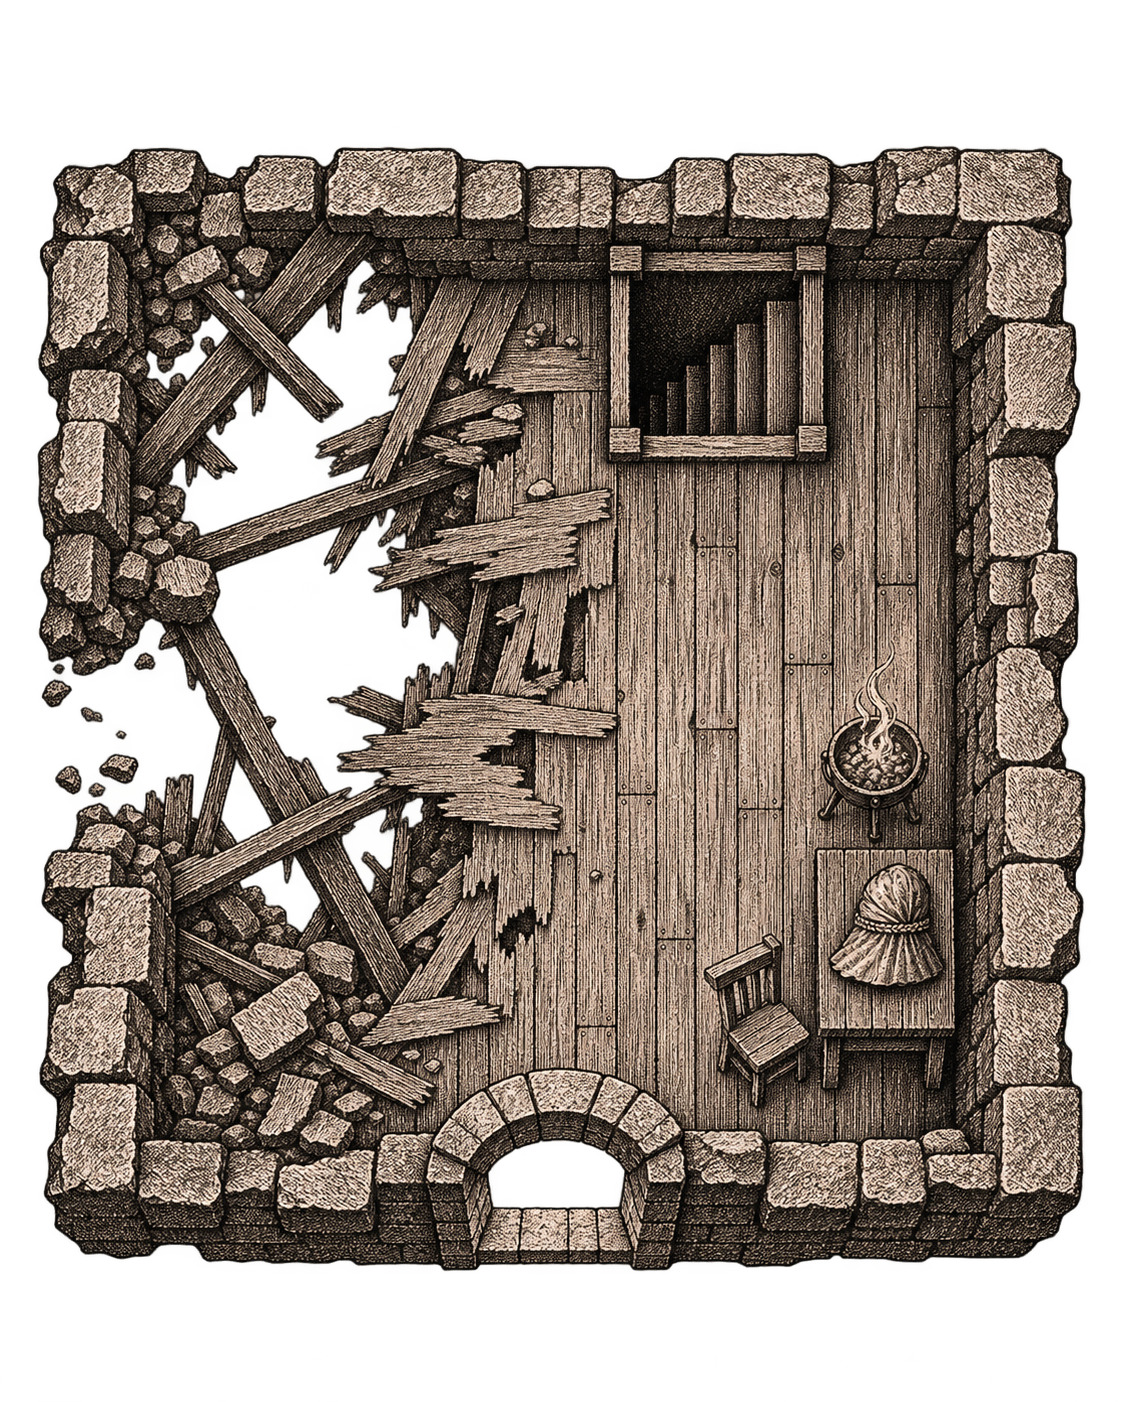
\includegraphics[width=.98\linewidth,height=70mm,keepaspectratio]{assets/hollow-hearth/map-upper.jpg}\par\vspace{2pt}
{\footnotesize\itshape\color{rpgbrown}Vieille tour de guet~: étage\par}
{\scriptsize Escalier au nord~; côté ouest à découvert~; fenêtre sud, cloche et brasero du côté est intact.\par}
&
\centering\vspace{0pt}
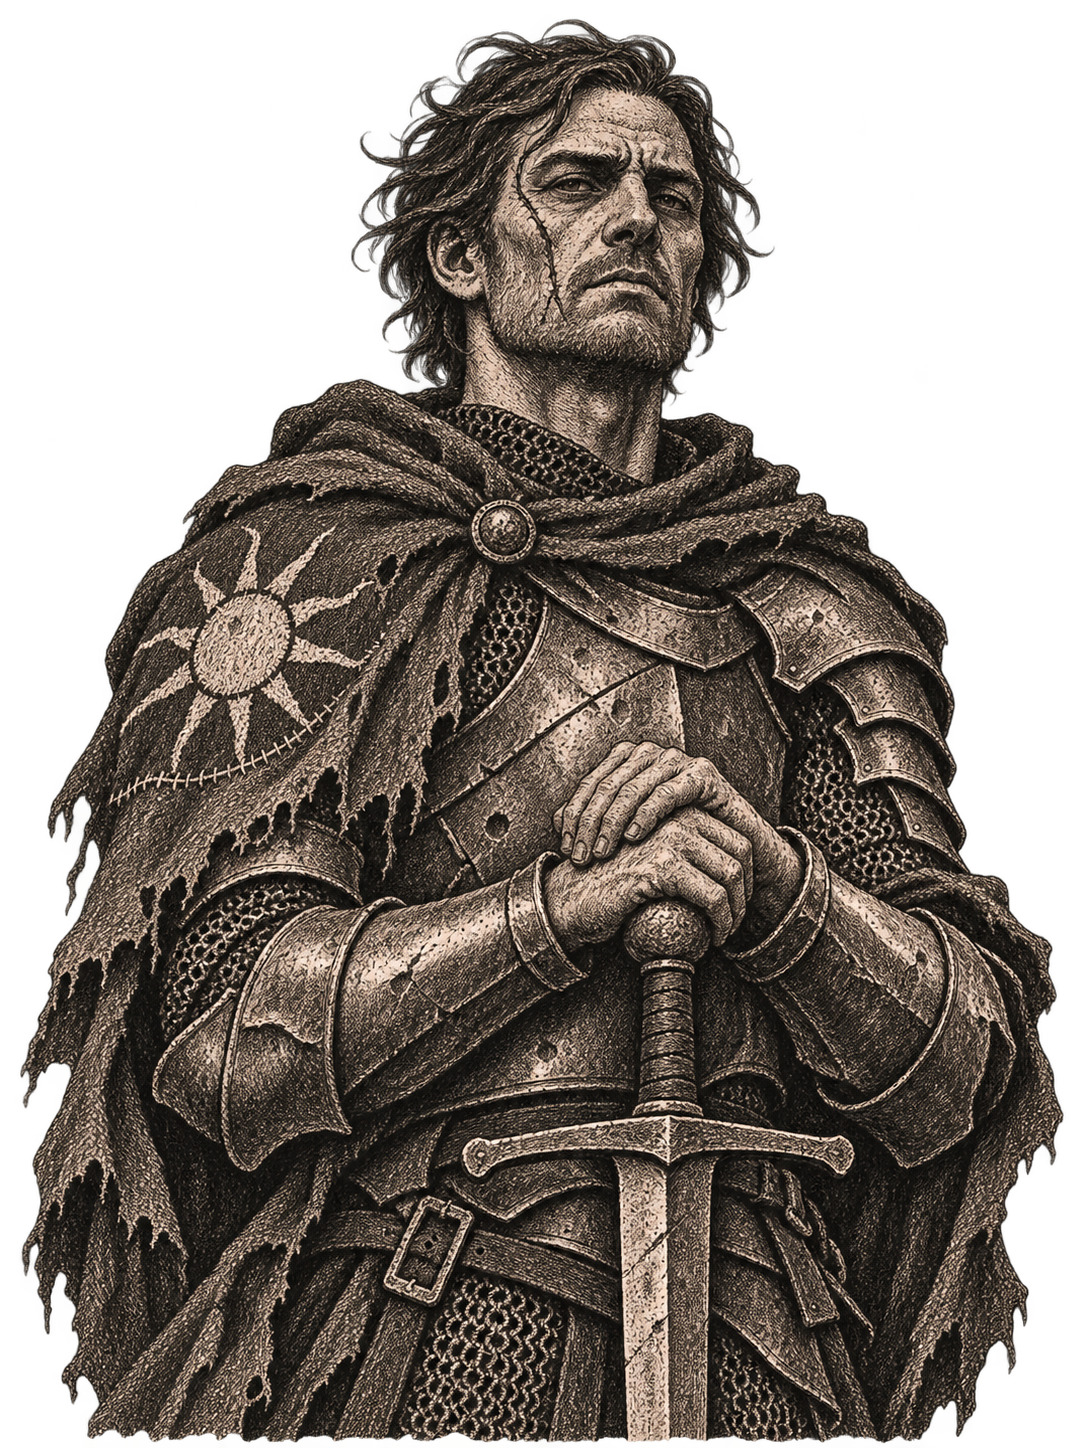
\includegraphics[width=.95\linewidth,height=68mm,keepaspectratio]{assets/hollow-hearth/corwin.jpg}\par\vspace{2pt}
{\footnotesize\itshape\color{rpgbrown}Sir Corwin Vask\par}
\end{tabular}
\par\medskip

Sir Corwin est assis sur une chaise de bois près de la \textbf{fenêtre sud}, et surveille le chemin par lequel l’acheteur montera. La cloche repose à côté de lui sur une petite table, toujours enveloppée dans sa toile huilée maculée de boue. Un brasero aux braises faibles fournit la seule lumière chaude de la pièce. L’escalier débouche contre le mur nord, \textbf{derrière lui}.

La \textbf{moitié ouest de l’étage est à ciel ouvert}~: l’effondrement qui a emporté le mur ouest du rez-de-chaussée a aussi emporté le toit ouest et une partie du plancher ouest. Des poutres détachées pendent de travers. Le plancher ouest à découvert est dangereux à traverser sans précaution.

Cela crée une \textbf{quatrième approche}, que le texte précédent ne faisait que suggérer~:

\textbf{L’escalade.} Un personnage qui possède \textbf{Acrobatie} peut gravir l’éboulis du mur effondré au rez-de-chaussée, puis continuer par l’extérieur du mur ouest éventré pour entrer par la brèche du toit. Lancez \textbf{Dextérité + Acrobatie, SD~4} pour grimper proprement~; sans Acrobatie, \textbf{SD~5}. Un échec signifie une chute~: 1~Blessure due à la hauteur, plus le bruit de la chute (Corwin l’entendra). En cas de réussite, le personnage se laisse tomber à l’étage \emph{derrière} Corwin et le prend par surprise. Cette approche ne concerne qu’un seul personnage~: le Guerrier en armure lourde ne peut pas faire cette escalade, et le Mystique à 2~PV ne peut pas se permettre la chute en cas d’échec. \textbf{Un Aventurier agile est le mieux placé pour cette approche.}

\par\Needspace{12\baselineskip}\noindent\textbf{Éléments tactiques de l’étage~:}

\begin{itemize}
\tightlist
\item
  \textbf{La fenêtre sud.} Quiconque atteint la cloche peut la jeter dehors --- elle s’écrase près du feu de camp en contrebas, peut-être fêlée. L’acheteur, qui observe depuis le chemin, le verra. Un Protagoniste peut aussi s’enfuir par la fenêtre en sautant jusqu’au sol (Dextérité + Acrobatie, \textbf{SD~4} pour atterrir proprement~; un échec coûte 1~Blessure).
\item
  \textbf{La moitié ouest instable.} Tout combat qui se déroule sur la partie effondrée subit une Condition~: \textbf{$-1$ degré}. Un personnage poussé par-dessus le bord tombe d’un étage (2~Blessures). Corwin, qui connaît la pièce, ne combat que sur la moitié est --- et tentera volontiers de pousser ses ennemis vers le plancher dangereux.
\item
  \textbf{Le brasero.} Renversé, il répand ses braises sur le plancher de bois sec --- le feu se propage en l’équivalent de deux scènes d’action, et la pièce devient invivable. Un geste désespéré, à la portée de tous, qui peut sauver le groupe ou détruire la cloche avec tout le reste.
\item
  \textbf{L’armure lourde de Sir Corwin.} Son armure lourde fixe le SD pour le toucher à \textbf{4 avec la Force} ou à \textbf{5 avec la Dextérité}. Elle ne réduit pas les dégâts. Un brasero renversé, une poussée vers le bord effondré, ou un Critique obtenu par un Protagoniste qui a déclaré un Effort peuvent changer le cours de l’affrontement.
\end{itemize}

\subsubsection{Adapter l’affrontement}\label{adapter-laffrontement}

\begingroup\setlength{\arrayrulewidth}{.34pt}\arrayrulecolor{rpgline}\renewcommand{\arraystretch}{1.32}\rowcolors{2}{rpgshade}{white}\par\smallskip\noindent\begin{tabularx}{\linewidth}{|Y|Y|Y}\hline
\rpghead{Taille du groupe} & \rpghead{Brigands} & \rpghead{Sir Corwin} \\ \hline
3 joueurs & 3 brigands (en groupe) & Oui \\ \hline
4 joueurs & 4 brigands (2 dehors, 2 dedans) & Oui \\ \hline
\end{tabularx}\arrayrulecolor{black}\endgroup\par\smallskip

Si le groupe semble en grande difficulté, faites fuir un brigand au premier signe de véritable effusion de sang. S’il traverse la scène sans peine, l’acheteur arrive en avance.

\subsubsection{Le retournement · L’acheteur}\label{le-retournement-lacheteur}

Si le groupe se trouve encore à la tour de guet à \textbf{minuit} --- en plein combat, en pleine discussion ou après avoir vaincu ---, une silhouette en robe sort du bois, seule, sans visage sous sa capuche. \textbf{L’acheteur est un membre du Peuple Creux sous apparence humaine.} Il veut que la cloche se taise à jamais, pas qu’elle soit détruite. Il apporte une petite bourse d’argent. Il parle avec ces mêmes voix, pas tout à fait justes, que le groupe a entendues à demi en entrant dans le bois.

\par\smallskip\begin{rpgnote}[fontupper=\normalfont]\textbf{L’acheteur (membre du Peuple Creux sous apparence humaine)} \emph{SD F3/D4 · Expert · 4~Blessures · toucher (1F Merveille~; sur un Critique, 2B et une Condition qui dure jusqu’à la fin de la scène) · sans armure.} \emph{Comportement~: «~Prononce les mauvaises syllabes. Les arbres ne répondent pas. Saigne de la sève, pas du sang.~»}\end{rpgnote}\par\smallskip
C’est un \textbf{moment de choix}. Le groupe peut~:

\begin{itemize}
\tightlist
\item
  \textbf{Refuser et combattre.} \emph{(Caractéristiques ci-dessus.)}
\item
  \textbf{Accepter l’argent.} Le groupe repart riche. On ne reverra plus jamais l’Âtre Creux vivant. \emph{Si les joueurs font ce choix, faites-en une véritable fin.}
\item
  \textbf{Mentir et tendre une embuscade à l’acheteur.} \textbf{Jets de Savoir opposés au Savoir (Expert) de l’acheteur}. Si le groupe l’emporte, il garde l’argent \emph{et} la cloche --- mais le bois l’a marqué, et l’aventure suivante commence avec cette marque.
\end{itemize}

\subsubsection{L’apogée --- et le dernier lancer}\label{lapoguxe9e-le-dernier-lancer}

Quelle que soit la voie choisie, le moment culminant devrait laisser au moins un Protagoniste dans l’état \textbf{Amoché} ou \textbf{Grave}. Surveillez les PV à la table. Dès qu’un joueur tombe à \textbf{1~PV} et qu’il lui reste un jet à faire pour terminer la scène --- faites une pause. Regardez-le droit dans les yeux, par-dessus la table. Demandez~:

\begin{quote}
\emph{«~On en est au dernier lancer. Veux-tu saigner pour ça~?~»}
\end{quote}

Guidez-le dans la déclaration d’un \textbf{Effort} \emph{(manuel, p.~13)}. Laissez-le lancer les dés~; la Blessure de Fatigue vient après le jet. \textbf{C’est le moment qui donne son nom au jeu.} Faites-le sentir. Si le jet réussit, la table devrait exulter. S’il échoue, la table devrait se taire.

\par\vspace{3pt}

\subsection{Résolution}\label{ruxe9solution}

Trois fins nettes, avec des conséquences qui préparent l’aventure suivante~:

\textbf{La cloche revient.} Hesta remet la \textbf{Lame de sel} et offre toute l’hospitalité du village. Si sa fleur a été rapportée, Vela compte le groupe parmi ses amis. La nouvelle se répand jusqu’à la ville suivante. \emph{L’aventure suivante commence quand quelqu’un vient chercher le groupe en le nommant.}

\textbf{La cloche est réduite au silence ou vendue.} Le groupe repart riche et marqué. Le Peuple Creux l’a remarqué. \emph{Une aventure future commence par des murmures nocturnes qui connaissent leurs noms.}

\textbf{La cloche est détruite.} Que ce soit par un Contrecoup malheureux ou par un combat désespéré, le Peuple Creux revient à l’Âtre Creux la nuit sans lune. \emph{L’aventure suivante commence quand le groupe tente de réparer le mal. Veyl Ashen, le Mystique d’origine, n’est peut-être pas aussi mort que le prétendent les chroniques.}

\subsubsection{Les trois questions}\label{les-trois-questions}

Terminez la séance en faisant répondre le groupe, ensemble, aux trois questions de Progression (manuel, p.~11). Un bilan honnête, et non généreux, est le bon. Un nouveau joueur qui s’est bloqué à chaque occasion n’a gagné aucun point de progression. Un nouveau joueur qui a essayé, échoué et assumé les conséquences en a gagné trois. Expliquez-le clairement, avec douceur, la première fois.

\par\vspace{3pt}

\par\smallskip\section*{Aide-mémoire du Narrateur}\addcontentsline{toc}{section}{V. Aide-mémoire du Narrateur}
\begingroup\footnotesize\setlength{\arrayrulewidth}{.34pt}\arrayrulecolor{rpgline}\renewcommand{\arraystretch}{1.14}
\noindent\begin{minipage}[t]{.49\linewidth}
\begin{tabularx}{\linewidth}{|>{\hsize=.78\hsize}Y|>{\hsize=1.22\hsize}Y|}\hline
\rpghead{Situation} & \rpghead{Règle / seuil} \\ \hline
SD 3–6 & Simple / Ordinaire / Difficile / Extrême \\ \hline
Distances & Au contact~; Proche~; À portée~; Loin \\ \hline
Aide & Expert ou plus~: +1d6~; en dessous~: +1d6 et SD +1 \\ \hline
Effort & +1d6 avant le jet~; 1F après \\ \hline
État & $\le$ 2~PV~: $-1$ degré~; $\le$ 1~PV~: $-2$ degrés \\ \hline
\end{tabularx}
\end{minipage}\hfill
\begin{minipage}[t]{.49\linewidth}
\begin{tabularx}{\linewidth}{|>{\hsize=.78\hsize}Y|>{\hsize=1.22\hsize}Y|}\hline
\rpghead{Situation} & \rpghead{Règle / seuil} \\ \hline
Pont & Dextérité SD~4~; corde SD~3~; chute 2B \\ \hline
Pistage & Dextérité + Survie, SD~4 \\ \hline
Discrétion & Dextérité + Discrétion, SD~4 \\ \hline
Escalade & Dextérité + Acrobatie, SD~4 (sinon 5) \\ \hline
Corwin & SD F4/D5~; Expert~; 6B~; épée 2B \\ \hline
\end{tabularx}
\end{minipage}
\arrayrulecolor{black}\endgroup


\HHAdventureBackCover
\end{document}
